%************************************************
\chapter{Theoretical background}
\label{ch:theory}
%************************************************

\section{Introduction}
Particle physics is a branch of physics that studies the most fundamental particles and their interactions.
All matter in the universe is made up of these fundamental particles, and their interactions are described by the theories in particle physics.
In 20th century, our understanding about the nature of fundamental particles has had great breakthrough and  advance.
Also, many particle colliders have been built to give much insight to develop the theories and test the theories.
The currently mainstream theory of particle physics is called the Standard Model.

\section{Standard Model}
\label{sec:Standard_Model}
Standard Model(SM) is the current theory to describe the fundamental particles in particle physics.
It has already gained huge success in predicting the experimental results, including the prediction of existence of the top quark, the tau neutrino, and the Higgs boson.
It has also explained the most experimental results with high accuracy.
It represents our best understanding of how the fundamental particles interact with each other.

Physicists discovered that there are 4 fundamental forces in the universe: electromagnetic force, weak force, strong force, and gravitational force.
SM can describe three of them: electromagnetic, weak and strong interaction.
Figure \ref{fig:SM_particles} shows all fundamental particles in the SM, and their mass, electric charge and spin.
All matter is made up of fermions (purple and green), which is the first 3 columns in figure \ref{fig:SM_particles}.
Fermions are divided into two groups: quarks(purple) and leptons(green).
The forces between the fermions are mediated by the force carriers, which is gauge bosons(red).
Higgs bosons(yellow) are scalar bosons, which explain the masses of other massive particles.

\begin{figure}
\centering
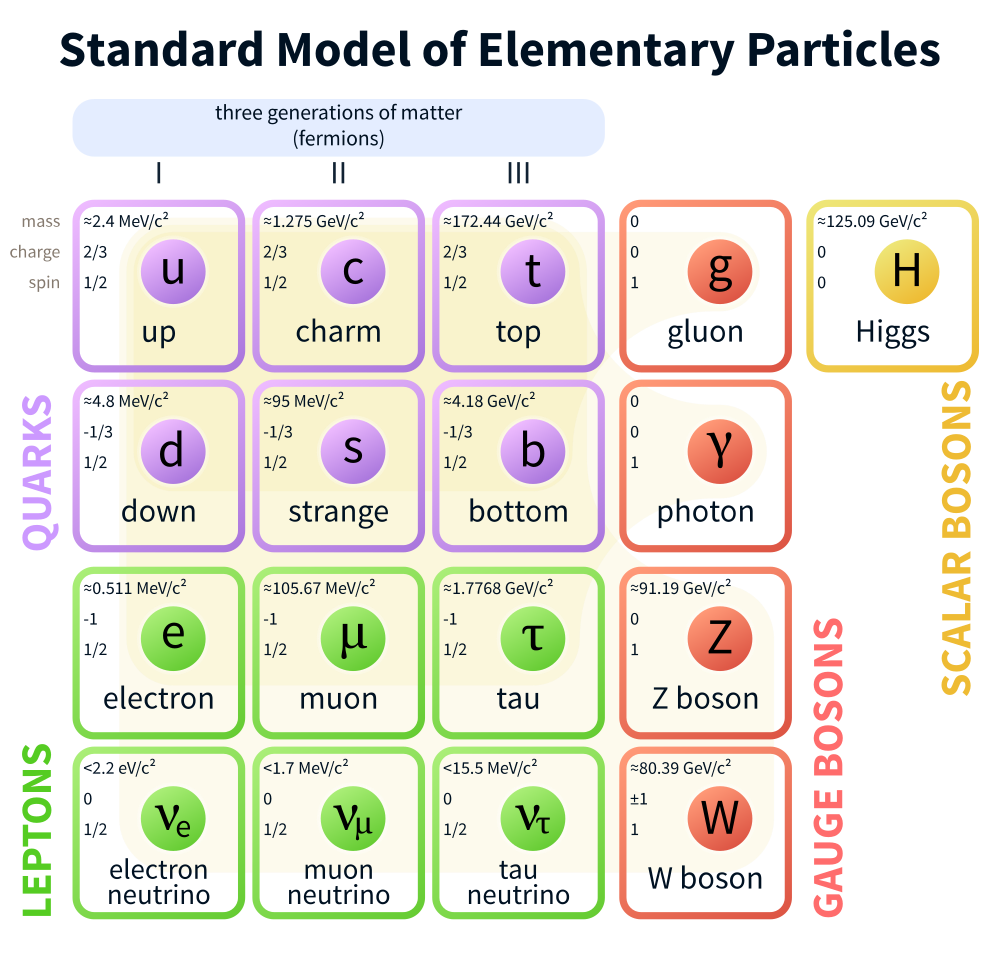
\includegraphics[width=\textwidth]{data/photo/theory/SM_particles.png}
\caption{The table for all fundamental particles in SM. \cite{SM_particles}}
\label{fig:SM_particles}
\end{figure}

\subsection{Matter particles}
There are six types of quarks: up quarks(u), down quarks(d), charm quarks(c), strange quarks(s), top quarks(t) and bottom quarks(b).
Quarks interact with strong interactions, while leptons do not.
There are three types of charged leptons: electrons, muons and taus.
There are three types of neutral leptons: electron neutrinos, muon neutrinos and tau neutrinos.
The first column is the first generation, which is the lightest and the most stable particles.
Hence, normal matter in our daily life is made from the particles in the first generation.
The second and third column are the second and third generation respectively, which are heavier and less stable particles.
These particles will finally decay into the particles in the first generation.
Due to the phenomenon of neutrino oscillation, neutrinos are massive, but their value are still unknown.

\subsection{Forces and carrier particles}
Photon is the force carrier of electromagnetic interactions.
Gluon is the force carrier of strong interactions.
Z and W bosons are the force carriers of weak interactions.
The effects of these fundamental forces stem from the exchange of the corresponding force carrier.
These forces also have different strengths and different interaction ranges.
The strong force is the strongest force, the electromagnetic force is in the middle, and the weak force is the weakest force.
The electromagnetic force has infinite range, while the strong and weak forces have very short ranges at the level of subatomic particles.

For example, a proton is composed of two up quarks and one down quark, and a neutron is composed of one up quark and two down quarks.
The forces between quarks inside the proton are mediated by gluons.

\subsection{Feynman diagram}
The fundamental interactions among these fundamental particles are described by the allowed Feynman vertices.
All these allowed Feynman vertices in the SM are shown in figures \ref{fig:vertices_SM} and \ref{fig:vertices_higgs}.

\begin{figure}
\centering
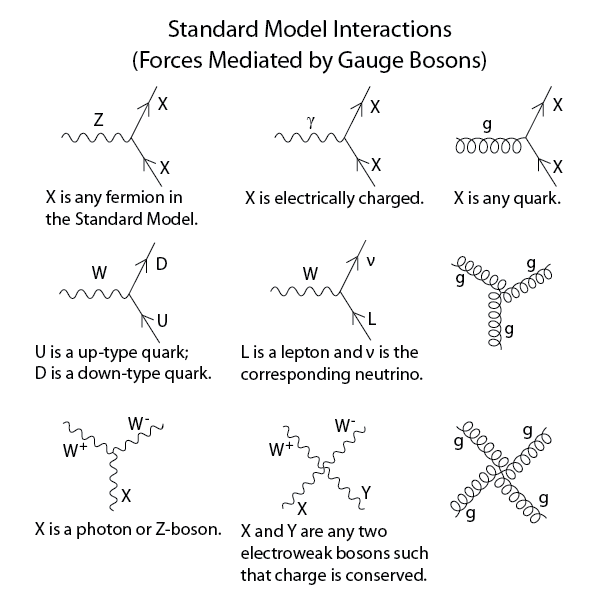
\includegraphics[width=\textwidth]{data/photo/theory/vertices_SM.png}
\caption{All allowed fundamental Feynman vertices in SM, except higgs-related vertices. \cite{vertices_SM}}
\label{fig:vertices_SM}
\end{figure}

\begin{figure}
\centering
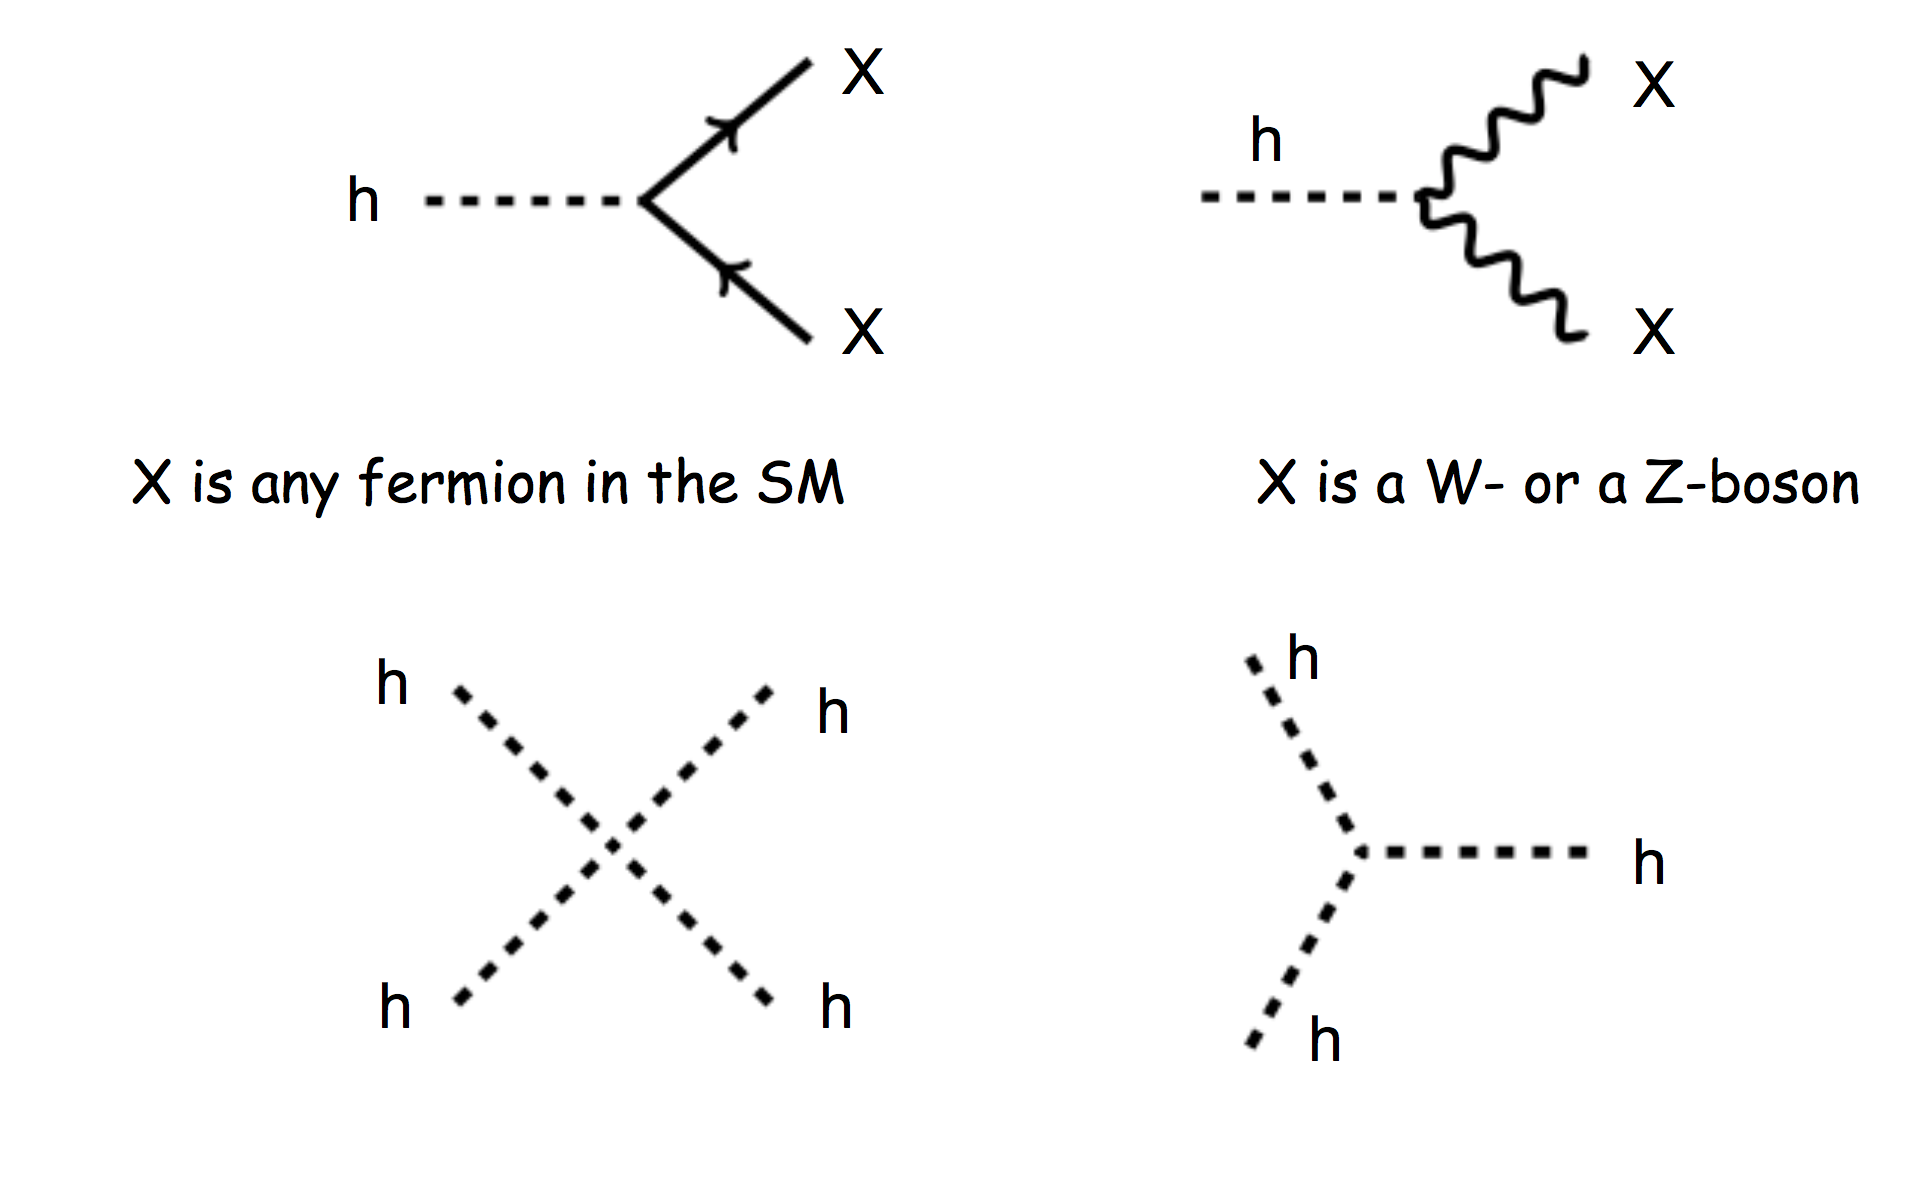
\includegraphics[width=\textwidth]{data/photo/theory/vertices_higgs.png}
\caption{All allowed fundamental higgs-related Feynman vertices in SM.}
\label{fig:vertices_higgs}
\end{figure}

\section{Limitation of Standard Model}
\label{sec:Limitation_Standard_Model}
Although the Standard Model can explain almost all experimental results, there are still some phenomena it cannot explain.

\subsection{Dark matter}
\label{sec:dark_matter}
Dark matter is some unknown matter that does not involve in electromagnetic interaction, but involves in gravitational interaction.
It was first discovered in the Milky Way, by studying the speed of the stars orbiting around the center of the Milky Way.
Because it does not involve in electromagnetic interaction, it cannot be seen by our telescopes.
However, the SM cannot explain what dark matter is.

\subsection{Hierarchy problem}
\label{subsec:hierarchy_problem}
The hierarchy problem is the question why the weak force is stronger than the gravitational force by $10^{24}$ times.
It is also asked why the mass of Higgs boson ($\sim 125$ GeV) is much lighter than the Planck mass ($\sim 10^{19}$ GeV).

The Lagrangian for the interaction term between the fermion Dirac field $f$ and the Higgs field $H$ (i.e. Yukawa interaction) is given by
\begin{equation}
\mathcal{L}_{\text{Yukawa}} = - \lambda_f \bar{f} H f
\end{equation}
where $\lambda_f$ is the Yukawa coupling constant.
The quantum correction to the square of the Higgs mass $\Delta m^2_H$ is then given by \cite{primer}
\begin{equation}
\Delta m^2_H = - \frac{|\lambda_f|^2}{8 \pi^2} \Big[ \Lambda^2 - 3 m_f^2 \ln \Big( \frac{\Lambda}{m_f} \Big) \Big] + \dots
\label{eq:higgs_correction}
\end{equation}
where $\Lambda$ is the energy scale up to which the quantum effects of gravity are not dominant, namely the Planck scale ($\sim 10^{19}$ GeV).
Because the first term is quadratic divergent in $\Lambda$, its correction to the Higgs mass is in the order of Planck scale.
Unless there are very delicate cancellation between the correction terms, the Higgs mass should be in the order of Planck scale.
But, we found that the experimental Higgs mass is in the order of 125 GeV, and this is called the hierarchy problem.

\subsection{Unification of forces}
In the 1860s, James Clerk Maxwell wrote down his famous equations Maxwell's equations, which unify two different phenomena: electricity and magnetism.
Due to this unification, we now understand that electricity and magnetism are two different manifestations of the same phenomenon, and we now call it electromagnetism.

Similar thing happened in the 1970s, physicists developed a theory that unified two fundamental forces: electromagnetic force and weak force.
At the energy scale above 246 GeV, these two forces will merge into a single force: electroweak force.
This unification predicted the existence of weak neutral current and a force carrier to carry this weak force.
This force carrier Z boson was later confirmed experimentally in CERN.

After that, an effect of strong force was found experimentally that the strong force becomes weaker when the energy scale is higher.
This may indicate that electroweak force and strong force will become a single force at higher energy scale.
There are some theories beyond the Standard Model that can unify these forces, such as supersymmetry.

\section{Supersymmetry}
Supersymmetry(SUSY) is a theoretical extension of the Standard Model, and can answer some questions which the Standard Model cannot answer, mentioned in section \ref{sec:Limitation_Standard_Model}.
One of the problems SUSY can solve is the hierarchy problem of Higgs mass mentioned in section \ref{subsec:hierarchy_problem}.
We first notice that the negative sign of the quadratic divergent term in the equation \ref{eq:higgs_correction} is due to the correction from the fermions.
If there is a symmetry between the fermions and bosons, and the quadratic terms due to the bosons cancel with the quadratic terms due to the fermions, the hierarchy problem can be solved.
This new symmetry is called the supersymmetry (SUSY).

\subsection{Minimal Supersymmetric Standard Model}
Minimal Supersymmetric Standard Model(MSSM) is the simplest realization of the supersymmetric theory that contains the minimum number of new particles and new interactions.
It predicts that each particle in the Standard Model has its own partner particle, called the superpartner, as shown in figure \ref{fig:SUSY_particles}.
This is the new symmetry between the fermions and bosons.
The name scheme for the superpartner of a fermion is to add a prefix ``s'', in front of the name of the original Standard Model particle: squarks and sleptons, etc.
For example, the superpartner of an electron is called selectron.
For the superpartner of a Standard Model boson, the suffix ``ino'' is added: gluino and Higgsino, etc.
As for the symbol for the superpartner, a tilde is added above the original symbol.
For example, the symbol for selectron is $\tilde{e}$.
Also, the spin of the superpartner differs from the Standard Model particle by 1/2.
For fermions, the spin of their superpartner is 0, while for bosons, the spin of their superpartner is 1/2.
The superpartners interact with the same forces as the Standard Model particles, but they have different masses.

\begin{figure}
\centering
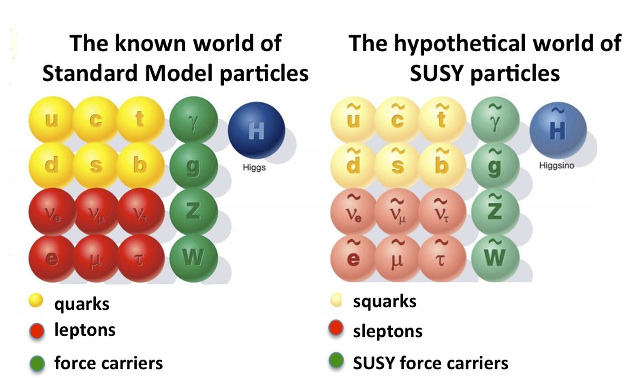
\includegraphics[width=\textwidth]{data/photo/theory/SM-SUSY-diagram.jpg}
\caption{The particles in Standard Model and their corresponding superpartners and their names}
\label{fig:SUSY_particles}
\end{figure}

The quantum correction terms from the superpartners cancel the quadratic divergent terms in the Higgs mass.
The idea is to postulate two scalar fields $\tilde{f}$ for each fermion, with the coupling constant to the Higgs $\lambda_{\tilde{f}}$.
\begin{equation}
\mathcal{L} = - \lambda_{\tilde{f}} |H|^2 |\tilde{f}|^2
\end{equation}
The quantum correction to the square of the Higgs mass $\Delta m^2_H$ for the scalar field is given by \cite{primer}
\begin{equation}
\Delta m^2_H = \frac{ \lambda_{\tilde{f}} }{16 \pi^2} \Big[ \Lambda^2 - 2 m_{\tilde{f}}^2 \ln \Big( \frac{\Lambda}{m_{\tilde{f}}} \Big) \Big] + \dots
\label{eq:higgs_correction2}
\end{equation}
The quadratic terms in \ref{eq:higgs_correction} and \ref{eq:higgs_correction2} exactly cancel with each other, if $\lambda_{\tilde{f}} = |\lambda_f|^2$.
The logarithmic terms are left in the correction terms for the Higgs mass.
Therefore, the hierarchy problem is solved.

In the MSSM, two neutral Higgs bosons ($H^0_u$ and $H^0_d$) and two charged Higgs bosons ($H^+_u$ and $H^-_d$) are introduced.
Therefore, there are 4 neutral bosons: $\gamma$, $Z$, $H^0_u$, $H^0_d$ and 4 charged bosons: $W^+$, $W^-$, $H^+_u$ ,$H^-_d$.
The superpartners of the four neutral bosons together form four mass eigenstates called neutralinos: $\tilde{\chi}_1^0$, $\tilde{\chi}_2^0$, $\tilde{\chi}_3^0$ and $\tilde{\chi}_4^0$.
The superpartners of the four charged bosons together form two mass eigenstates with electric charge $\pm 1$, called charginos: $\tilde{\chi}_1^\pm$ and $\tilde{\chi}_2^\pm$.
The subscripts of the symbol of the neutralinos and charginos are labeled by the ascending order in mass.
Table \ref{tab:SUSY_particle} summarizes the Standard Model particles and their superpartners.

\begin{table}[htbp]
\tiny
\centering
\begin{tabular}{|c|cccc|cccc|}
\hline
\hline
Type & SM particle & Symbol & Spin & R-parity & Superpartner & Symbol & Spin & R-parity \\
\hline
\hline
Fermions & Quark  & $q$ & $\frac{1}{2}$ & +1 & Squark  & $\tilde{q}$ & 0 & -1 \\
         & Lepton & $l$ & $\frac{1}{2}$ & +1 & Slepton & $\tilde{l}$ & 0 & -1 \\
\hline
Gluon & Gluon  & $g$ & $1$ & +1 & Gluino & $\tilde{g}$ & $\frac{1}{2}$ & -1  \\
\hline
Neutral EW Bosons & Photon         & $\gamma$ & $1$ & +1
                  &  &  &  &  \\
                  & Z Boson        & $Z$      & $1$ & +1
                  & Neutralinos & $\tilde{\chi}_1^0$, $\tilde{\chi}_2^0$, $\tilde{\chi}_3^0$, $\tilde{\chi}_4^0$ & $\frac{1}{2}$ & -1 \\
                  & Neutral Higgs  & $H^0_u$, $H^0_d$  & $0$ & +1
                  &  &  &  &  \\
\hline
Charged EW Bosons & W Boson        & $W^+$, $W^-$  & $1$ & +1
                  & Charginos & $\tilde{\chi}_1^\pm$, $\tilde{\chi}_2^\pm$ & $\frac{1}{2}$ & -1 \\
                  & Charged Higgs  & $H^+_u$, $H^-_d$  & $0$ & +1
                  &  &  &  &  \\
\hline
\hline
\end{tabular}
\caption{The spin and R-parity for the Standard Model particles and their superpartners.}
\label{tab:SUSY_particle}
\end{table}

The baryon number $B$ is defined by $\frac{1}{3} (n_q - n_{\bar{q}})$, where $n_q$ is the number of quarks and $n_{\bar{q}}$ is the number of anti-quarks.
The lepton number $L$ is defined by $n_l - n_{\bar{l}}$, where $n_l$ is the number of leptons and $n_{\bar{l}}$ is the number of anti-leptons.
In the Standard Model and the experimental data, $B-L$ is conserved, but in MSSM, it is no longer conserved.
To keep this conservation and prevent the proton decay, the R-parity $P_R$ is introduced.
\begin{equation}
P_R = (-1)^{3(B-L)-2s}
\end{equation}
where s is the spin.
By this definition, all Standard Model particles have R-parity $+1$, and all supersymmetric particles have R-parity $-1$.
If the R-parity is conserved, the lightest supersymmetric particle (LSP) does not decay.
If the LSP is electrically neutral and interacts with matter only by the weak interaction and gravity, for example the lightest neutralinos $\tilde{\chi}_1^0$ or a sneutrino $\tilde{\nu}$, it can be a candidate for dark matter mentioned in section \ref{sec:dark_matter}.
In this analysis, the R-parity is assumed to be conserved, and the lightest neutralino $\tilde{\chi}_1^0$ is assumed to be the LSP.
Due to the conservation of R-parity, the supersymmetric particles can only be pair-produced, and eventually decay into Standard Model particles and the lightest neutralino $\tilde{\chi}_1^0$, i.e. the LSP.

\section{Signal scenario}
\label{sec:Wh_signal}
In the recent searches for the squarks and gluinos, the masses of gluinos and the first and second generation squarks are suggested to be larger than 1 TeV, while the upper mass limits of the third generation squarks are below 1 TeV \cite{gluinos}.
In this case, the direct pair production of electroweak gauginos (i.e. neutralinos and charginos) can be the dominant SUSY production process at the LHC, if the masses of the gluinos and squarks are significantly heavier than the low mass electroweak gauginos.
Based on the results in the Run-I analysis \cite{run1} at the center-of-mass energy $\sqrt{s} = 8$ TeV shown in figure \ref{fig:result_run1}, the electroweak pair production is a promising search at a higher center-of-mass energy $\sqrt{s} = 13$ TeV with Run-II using 2015 and 2016 data.

\begin{figure}
\centering
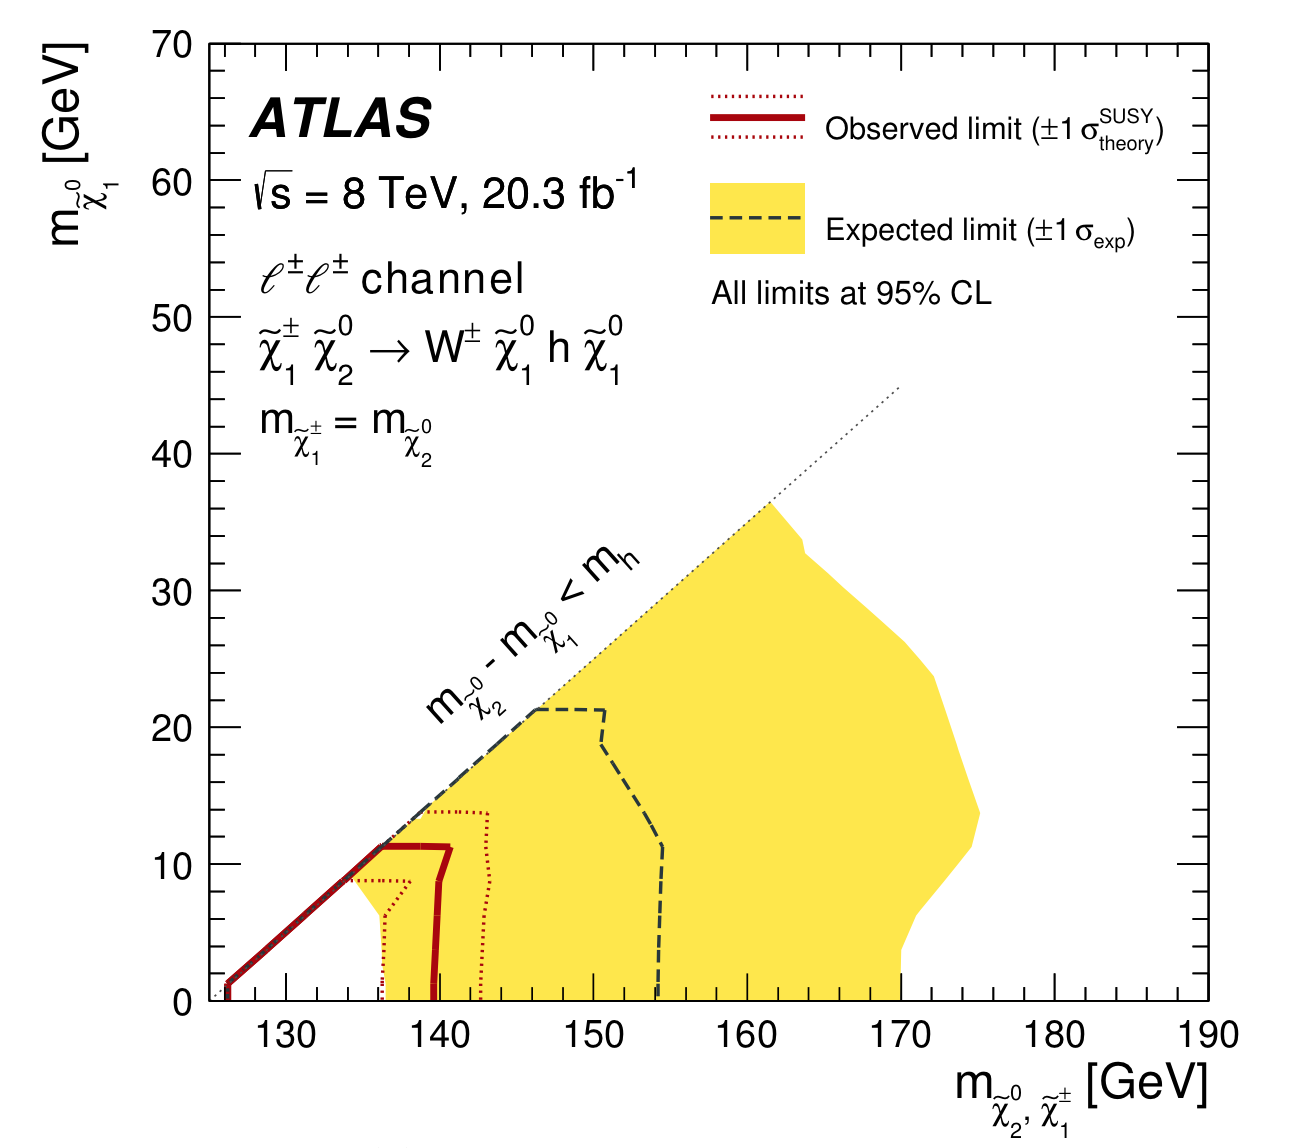
\includegraphics[width=0.5\textwidth]{data/photo/theory/run1.png}
\caption{The exclusion contours for the masses $m_{\tilde{\chi}_1^\pm , \tilde{\chi}_2^0}$ and $m_{\tilde{\chi}_1^0}$ in the Run-I analysis \cite{run1}.}
\label{fig:result_run1}
\end{figure}

The supersymmetric process searched in this thesis is the pair production of the lightest chargino $\tilde{\chi}_1^\pm$ and the second lightest neutralino $\tilde{\chi}_2^0$.
The masses of them are assumed to be the same, $m_{\tilde{\chi}_1^\pm} = m_{\tilde{\chi}_2^0}$, and denoted by $m_{\tilde{\chi}_1^\pm , \tilde{\chi}_2^0}$ in the following chapters.
With the assumption that all sleptons are heavier than $\tilde{\chi}_1^\pm$ and $\tilde{\chi}_2^0$,
$\tilde{\chi}_1^\pm$ decays to W boson and $\tilde{\chi}_1^0$ (i.e. $\tilde{\chi}_1^\pm \rightarrow W^{\pm} + \tilde{\chi}_1^0$)
and $\tilde{\chi}_2^0$ decays to the lightest MSSM Higgs boson $h$ and $\tilde{\chi}_1^0$ (i.e. $\tilde{\chi}_2^0 \rightarrow h + \tilde{\chi}_1^0$),
or Z boson and $\tilde{\chi}_1^0$ (i.e. $\tilde{\chi}_2^0 \rightarrow Z + \tilde{\chi}_1^0$).
In this thesis, we assume $\tilde{\chi}_1^\pm \rightarrow W^{\pm} + \tilde{\chi}_1^0$ and $\tilde{\chi}_2^0 \rightarrow h + \tilde{\chi}_1^0$ with 100\% branching ratio.
The mass of the lightest MSSM Higgs boson $h$ is set to be 125 GeV.

The W boson from $\tilde{\chi}_1^\pm$ decays into one lepton (electron or muon) and one neutrino (i.e. $W{^\pm} \rightarrow \ell^{\pm} + \nu$).
The Higgs boson from $\tilde{\chi}_2^0$ eventually decays into one lepton (electron or muon), quarks (i.e. jets) and neutrino(s) by various decay modes.
For example, $h \rightarrow W^{+} W^{-} $ and $h \rightarrow \tau^{+} \tau^{-} $ are the dominant decay modes, with one of the $W / \tau$ decays leptonically (e.g. $W{^\pm} \rightarrow \ell^{\pm} + \nu$) and another decays hadronically (e.g. $W \rightarrow q + q$).
Figure \ref{fig:signal_feynman} is the Feynman diagram for the signal process searched in this thesis.

\begin{figure}
\centering
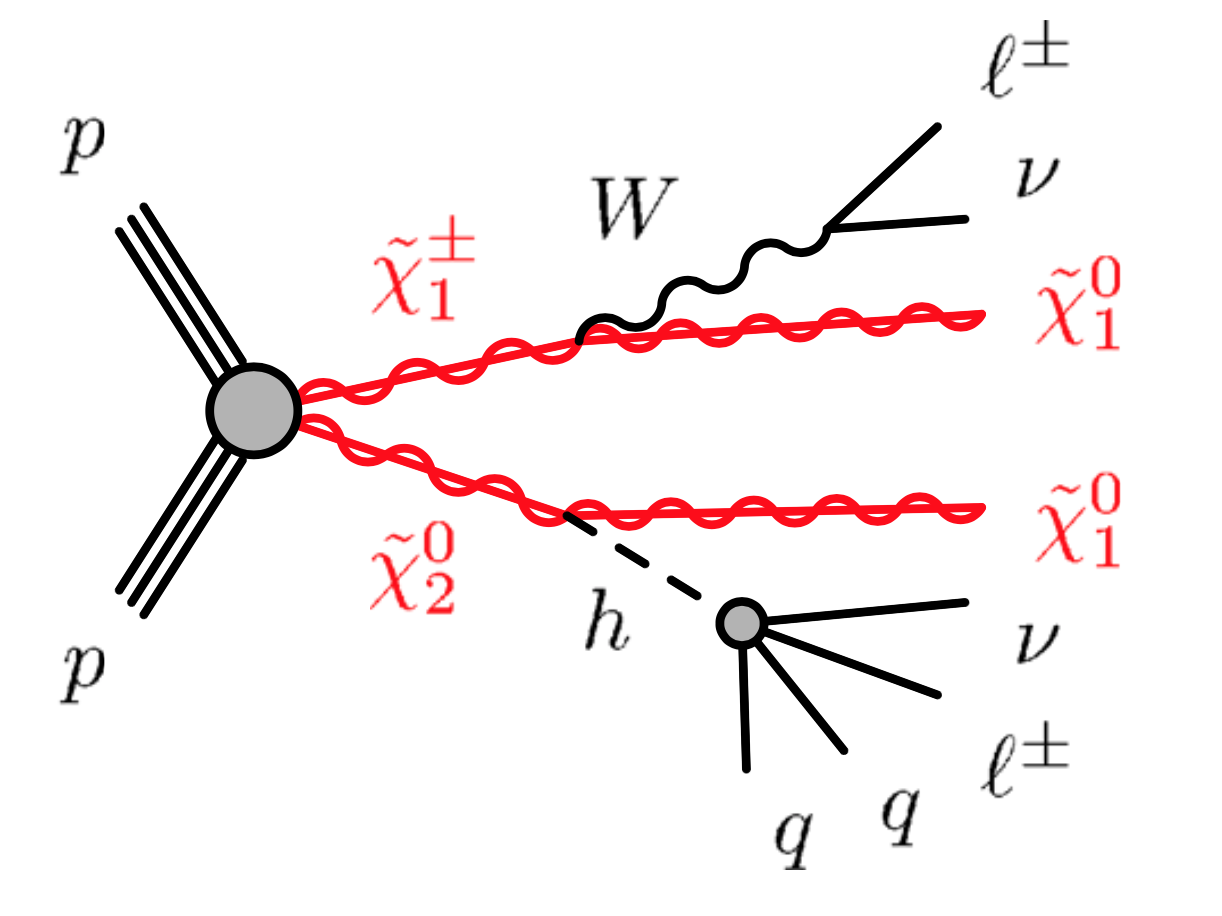
\includegraphics[width=0.5\textwidth]{data/photo/theory/signal_feynman.png}
\caption{The Feynman diagram for the Wh same-sign signal scenario in this thesis. The final states in this process include two same-sign leptons (electron or muon), quarks (i.e. jets) and missing transverse momentum contributed by the lightest neutralinos $\tilde{\chi}_1^0$ and neutrinos $\nu$.}
\label{fig:signal_feynman}
\end{figure}

The two leptons in the final states are either electrons or muons, and the term ``lepton'' (with symbol $\ell$) in the following chapters refers to electron or muon, but not tau lepton or neutrino.
We search for the final state with exactly two leptons with the same electric charge, which rarely exists in the Standard Model.
In the case that mass splitting is close to the mass of Higgs boson, which is called the compressed region, one of the lepton could be very soft that it fails the requirement of the signal lepton, due to the low momentum of the Higgs boson.
However, if the Higgs boson eventually decays into two leptons, for example $h \rightarrow ZZ$ with one of the Z boson decaying leptonically (e.g. $Z \rightarrow \ell^{+} + \ell^{-}$) and another decaying hadronically (e.g. $Z \rightarrow q + q$), the total number of leptons in the final state is three.
If one of the three leptons is soft and another two leptons have the same electric charge, this scenario will have the same final state as our signal.
This means that in the compressed region, our 2-leptons search channel would be more sensitive than the 3-leptons channel.

Because the two neutralinos $\tilde{\chi}_1^0$ and neutrinos $\nu$ in the final state cannot be detected, a large missing transverse momentum (i.e. unbalanced momentum in the detector) is expected.

This analysis is a collaborative work with other people and the results are mainly based on the paper \cite{Wh} and the internal note \cite{WhSS}.
